\documentclass[11pt]{article}
\usepackage[a4paper,margin=1in]{geometry}
\usepackage{amsmath,amssymb,amsthm}
\usepackage{tikz}
\usetikzlibrary{arrows.meta,calc}
\usepackage{xcolor}
\usepackage[hidelinks]{hyperref}
\hypersetup{pdftitle={Three tangent circles and a fair coin},pdfauthor={Vamshi Jandhyala}}
\setlength{\parskip}{0.4em}
\setlength{\parindent}{0pt}

\newtheorem{theorem}{Theorem}
\newtheorem{lemma}{Lemma}
\theoremstyle{remark}
\newtheorem*{remark}{Remark}

\definecolor{inkblue}{RGB}{40,76,105}
\definecolor{softblue}{RGB}{226,235,243}
\definecolor{softgray}{RGB}{236,236,236}
\definecolor{rust}{RGB}{153,70,45}
\definecolor{sand}{RGB}{246,226,205}

\title{Three tangent circles and a fair coin}
\author{Vamshi Jandhyala}
\date{}

\begin{document}
\maketitle
\vspace{-2em}

\begin{abstract}
Three circles touch in pairs, and a triangle is formed by choosing one point at random on
each. The triangle contains the incentre of the triangle of centres with probability exactly
$\frac12$, whatever the three radii. The proof rests on one lemma about two touching circles:
a random chord joining them crosses their common tangent at a point from which the two
centres are seen at an angle that is uniformly distributed. A refinement turns the pair of
random points into a uniform point on a sphere, on which each way of missing the incentre
becomes a lune.
\end{abstract}

\section{A ring of three circles}

Draw three circles, each touching the other two, and pick a point at random on each of them.
How often does the triangle of the three points contain the incentre of the triangle formed
by the centres? It is worth guessing before reading on, and a few sketches like
Figure~\ref{fig:ring} suggest that the answer is not obvious.

\begin{figure}[ht]
\centering
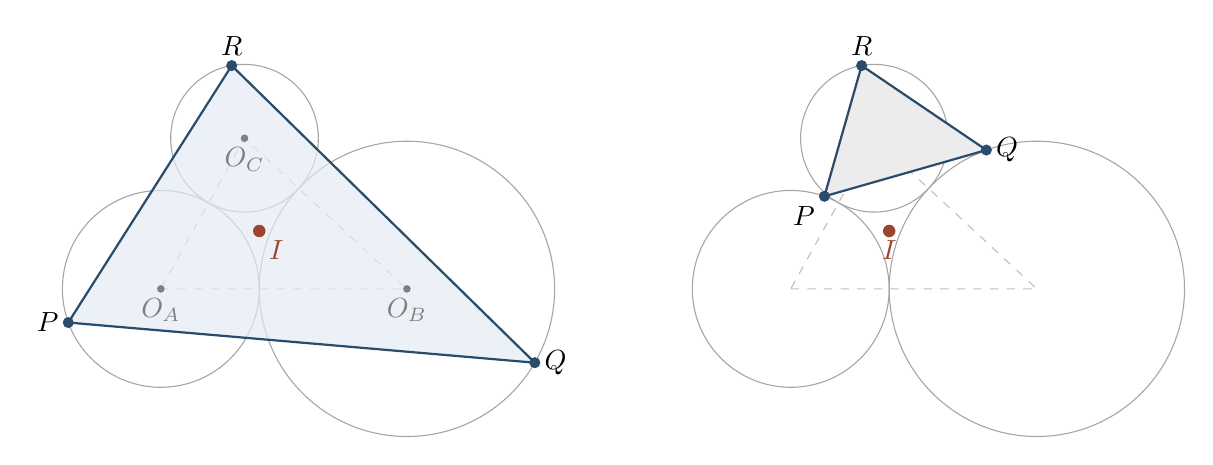
\begin{tikzpicture}[scale=1.25,line join=round]
  \coordinate (A) at (0,0); \coordinate (B) at (2.5,0); \coordinate (C) at (0.85,1.53);
  \coordinate (I) at (1.0,0.588);
  \draw[gray!70] (A) circle (1); \draw[gray!70] (B) circle (1.5); \draw[gray!70] (C) circle (0.75);
  \draw[gray!50,dashed] (A)--(B)--(C)--cycle;
  \coordinate (P) at (-0.940,-0.342); \coordinate (Q) at (3.799,-0.750); \coordinate (R) at (0.720,2.268);
  \fill[softblue,opacity=.7] (P)--(Q)--(R)--cycle;
  \draw[thick,inkblue] (P)--(Q)--(R)--cycle;
  \foreach \p in {P,Q,R} \fill[inkblue] (\p) circle (1.6pt);
  \fill[rust] (I) circle (1.8pt); \node[rust,below right] at (I) {$I$};
  \node[left] at (P) {$P$}; \node[right] at (Q) {$Q$}; \node[above] at (R) {$R$};
  \foreach \p/\n in {A/O_A,B/O_B,C/O_C} {\fill[gray] (\p) circle (1.1pt); \node[gray,below] at (\p) {$\n$};}
  \begin{scope}[xshift=6.4cm]
  \coordinate (A) at (0,0); \coordinate (B) at (2.5,0); \coordinate (C) at (0.85,1.53);
  \coordinate (I) at (1.0,0.588);
  \draw[gray!70] (A) circle (1); \draw[gray!70] (B) circle (1.5); \draw[gray!70] (C) circle (0.75);
  \draw[gray!50,dashed] (A)--(B)--(C)--cycle;
  \coordinate (P) at (0.342,0.940); \coordinate (Q) at (1.987,1.410); \coordinate (R) at (0.720,2.268);
  \fill[softgray] (P)--(Q)--(R)--cycle;
  \draw[thick,inkblue] (P)--(Q)--(R)--cycle;
  \foreach \p in {P,Q,R} \fill[inkblue] (\p) circle (1.6pt);
  \fill[rust] (I) circle (1.8pt); \node[rust,below] at (I) {$I$};
  \node[below left] at (P) {$P$}; \node[right] at (Q) {$Q$}; \node[above] at (R) {$R$};
  \end{scope}
\end{tikzpicture}
\caption{Radii $1$, $1.5$ and $0.75$. On the left the random triangle contains the incentre
$I$ of the triangle of centres $O_AO_BO_C$; on the right it does not.}
\label{fig:ring}
\end{figure}

The answer is a fair coin.

\begin{theorem}\label{thm:main}
For any three mutually tangent circles, with one uniform random point on each, chosen
independently, the triangle of the three points contains the incentre of the triangle of
centres with probability $\frac12$.
\end{theorem}

Dan asked this on Mathematics Stack Exchange for three equal circles~\cite{DanEqual}, and
there it was settled by an integral: Dan reduced it to a single integral, and user170231
evaluated it with a contour argument~\cite{user170231}. Dan then asked about unequal radii,
where simulations gave $\frac12$ again~\cite{DanAny}, and isolated a statement about two
circles that would explain it~\cite{DanLemma}. On MathOverflow~\cite{DanMO} he asked for a
proof that shows why the answer is $\frac12$. This note proves the theorem for all radii by
proving that two-circle statement, in the following form.

\begin{theorem}\label{thm:angle}
Two circles touch at $T$, and a chord $PQ$ joins a uniform random point $P$ of one to an
independent uniform random point $Q$ of the other. Let $Z$ be the point where $PQ$ crosses the
common tangent at $T$. Then $Z$ lies on either side of $T$ with probability $\frac12$, and the
angle $\theta=\angle O_AZO_B$ at which $Z$ sees the two centres is uniformly distributed on
$(\frac\pi2,\pi)$.
\end{theorem}

The angle is $\pi$ when $Z=T$, and it falls as $Z$ moves away; Theorem~\ref{thm:angle} says
that it falls at a uniform rate in probability. Seen this way the radii drop out entirely, and
that is why the final answer does not depend on them. Section~\ref{sec:sphere} shows that $\theta$
has a hidden partner: together they describe a uniform point on a sphere.

\section{What the incentre sees}

Let the circles have centres $O_A,O_B,O_C$ and radii $a,b,c$, and write $A,B,C$ for the angles of
the triangle of centres. Its sides are $b+c$, $c+a$ and $a+b$.

\begin{lemma}\label{lem:sectors}
The incircle of $O_AO_BO_C$ touches its sides at the three points where the circles touch.
Seen from its centre $I$, the three circles fill three angular sectors of widths $\pi-A$,
$\pi-B$, $\pi-C$, which tile the full turn.
\end{lemma}

\begin{proof}
The tangent from $O_A$ to the incircle has length
$\frac12\bigl((a+b)+(a+c)-(b+c)\bigr)=a$, so the incircle touches $O_AO_B$ at the point $T_C$
where the circles about $O_A$ and $O_B$ touch, and similarly at $T_A$ and $T_B$. The radius
$IT_C$ is perpendicular to $O_AO_B$, so the line $IT_C$ is the common tangent of those two
circles; likewise $IT_B$ is tangent to the circle about $O_A$. So from $I$, which lies outside
every circle, the circle about $O_A$ fills exactly the angle between the rays $IT_C$ and $IT_B$.
In the quadrilateral $O_AT_CIT_B$ two angles are right, so that angle is $\pi-A$. The three
widths add up to $3\pi-\pi=2\pi$, and adjacent sectors share a bounding ray.
\end{proof}

\begin{figure}[ht]
\centering
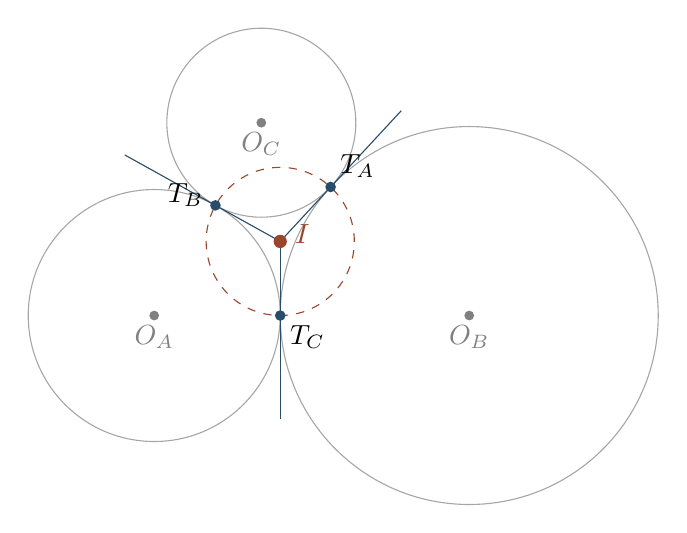
\begin{tikzpicture}[scale=1.6,line join=round]
  \coordinate (A) at (0,0); \coordinate (B) at (2.5,0); \coordinate (C) at (0.85,1.53);
  \coordinate (I) at (1.0,0.588);
  \coordinate (TA) at (1.400,1.020); \coordinate (TB) at (0.486,0.874); \coordinate (TC) at (1.0,0);
  \draw[gray!70] (A) circle (1); \draw[gray!70] (B) circle (1.5); \draw[gray!70] (C) circle (0.75);
  \draw[rust,dashed] (I) circle (0.588);
  \foreach \t in {TA,TB,TC} \draw[inkblue] (I) -- ($(I)!2.4!(\t)$);
  \foreach \t in {TA,TB,TC} \fill[inkblue] (\t) circle (1.2pt);
  \fill[rust] (I) circle (1.5pt); \node[rust,right] at ($(I)+(0.04,0.06)$) {$I$};
  \node[below right] at (TC) {$T_C$}; \node[above right] at (TA) {$T_A$}; \node[left] at ($(TB)+(-0.02,0.08)$) {$T_B$};
  \foreach \p/\n in {A/O_A,B/O_B,C/O_C} {\fill[gray] (\p) circle (1.1pt); \node[gray,below] at (\p) {$\n$};}
\end{tikzpicture}
\caption{The incircle (dashed) passes through the three contact points. The rays from $I$ through
them are common tangents, and they cut the turn around $I$ into the three sectors in which the
three circles are seen.}
\label{fig:sectors}
\end{figure}

So the directions of $P$, $Q$, $R$ seen from $I$ lie in three consecutive sectors
(Figure~\ref{fig:sectors}). The triangle $PQR$ contains $I$ exactly when each of the three gaps
between consecutive directions is less than $\pi$; the gaps add up to $2\pi$, so at most one of
them can be larger. When the gap between $P$ and $Q$ is the large one, say that the side $PQ$
\emph{misses} $I$.

\begin{lemma}\label{lem:miss}
The events ``$PQ$ misses $I$'', ``$QR$ misses $I$'' and ``$RP$ misses $I$'' are disjoint, and
their union is the event that $PQR$ does not contain $I$. The side $PQ$ misses $I$ exactly when
it crosses the common tangent $IT_C$ beyond $I$, on the side of $I$ away from $T_C$.
\end{lemma}

\begin{proof}
The first sentence is the remark above. The circles about $O_A$ and $O_B$ lie on opposite sides
of their common tangent, so $PQ$ crosses it at one point $Z$. As a point runs from $P$ to $Q$, its
direction from $I$ sweeps the angle $\angle PIQ<\pi$. If the gap from $P$ to $Q$ is less than
$\pi$, the swept angle is that gap, which contains the ray $IT_C$, so $Z$ lies on that ray. If
the gap is larger than $\pi$, the swept angle is the rest of the turn, which contains the
opposite ray, so $Z$ lies beyond $I$.
\end{proof}

So whether $PQ$ misses depends only on where $PQ$ crosses the tangent, and that is the subject of
Theorem~\ref{thm:angle}.

\section{Where a random chord crosses the tangent}

\begin{figure}[ht]
\centering
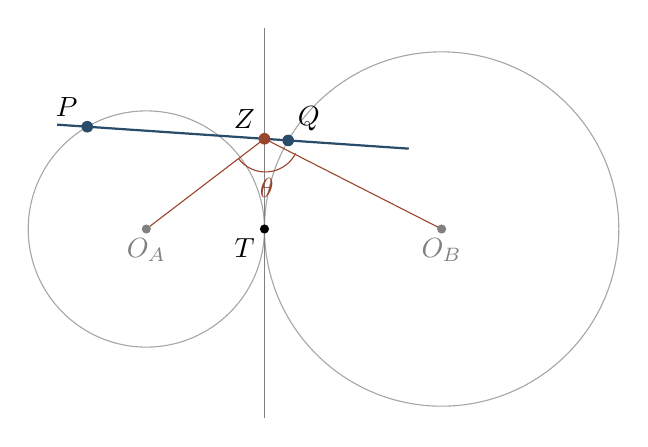
\begin{tikzpicture}[scale=1.5,line join=round]
  \coordinate (A) at (-1,0); \coordinate (B) at (1.5,0); \coordinate (T) at (0,0);
  \draw[gray!70] (A) circle (1); \draw[gray!70] (B) circle (1.5);
  \draw[gray] (0,-1.6) -- (0,1.7);
  \coordinate (P) at (-1.5,0.866); \coordinate (Q) at (0.201,0.75);
  \coordinate (Z) at (0,0.764);
  \draw[thick,inkblue] ($(P)!-0.15!(Q)$) -- ($(P)!1.6!(Q)$);
  \draw[rust] (A) -- (Z) -- (B);
  \draw[rust] ($(Z)!0.22!(A)$) arc[start angle={180+atan(0.764/1)}, end angle={360-atan(0.764/1.5)}, radius=0.287];
  \node[rust] at ($(Z)+(0.02,-0.42)$) {$\theta$};
  \foreach \p in {P,Q} \fill[inkblue] (\p) circle (1.4pt);
  \fill[rust] (Z) circle (1.4pt);
  \node[above left] at (P) {$P$}; \node[above right] at (Q) {$Q$}; \node[above left] at (Z) {$Z$};
  \fill (T) circle (1.1pt); \node[below left] at (T) {$T$};
  \fill[gray] (A) circle (1.1pt); \node[gray,below] at (A) {$O_A$};
  \fill[gray] (B) circle (1.1pt); \node[gray,below] at (B) {$O_B$};
\end{tikzpicture}
\caption{The chord $PQ$ meets the common tangent at $Z$, from which the centres are seen at the
angle $\theta$. As $Z$ climbs from $T$, $\theta$ falls from $\pi$ towards $\frac\pi2$, uniformly in
probability.}
\label{fig:chord}
\end{figure}

Put $T$ at the origin, the tangent on the $y$-axis, $O_A=(-a,0)$ and $O_B=(b,0)$, and let
$Z=(0,z)$. Write $p$ and $q$ for the angles that the segment $TZ$ subtends at the two centres, so
that
\begin{equation}\label{eq:pq}
  \tan p=\frac za,\qquad \tan q=\frac zb,\qquad \theta=\pi-p-q .
\end{equation}
Theorem~\ref{thm:angle} says that $s=p+q$ is uniform on $(-\frac\pi2,\frac\pi2)$; equivalently, $z$
has density
\begin{equation}\label{eq:density}
  f(z)=\frac1\pi\left(\frac{a}{a^2+z^2}+\frac{b}{b^2+z^2}\right),\qquad |z|<\sqrt{ab},
\end{equation}
which is the derivative of $s/\pi$. In words: the crossing point is spread like an even mixture
of the two Cauchy laws centred at $T$ with scales $a$ and $b$, cut off where the chords stop
reaching.

\begin{proof}[Proof of Theorem~\ref{thm:angle}]
We change variables from the pair of points to the line through them, and then count lines.

\emph{From points to lines.} Describe the line $PQ$ by its crossing height $z$ and its direction
$(\cos\omega,\sin\omega)$, with $|\omega|<\frac\pi2$. Moving $(z,\omega)$ by $(dz,d\omega)$ moves the
point of the line at signed distance $t$ from $Z$ sideways by $\cos\omega\,dz+t\,d\omega$. Where the
line cuts the first circle in a chord of half-length $c_A$, it meets the circle at an angle whose
sine is $c_A/a$, so the angular position $\alpha_P$ of $P$ on its circle changes by
$(\cos\omega\,dz+t_P\,d\omega)/c_A$; similarly for $Q$. The Jacobian determinant is therefore
\begin{equation}\label{eq:jacobian}
  d\alpha_P\,d\alpha_Q=\frac{\cos\omega\;|PQ|}{c_A\,c_B}\,dz\,d\omega .
\end{equation}
This is the classical density for pairs of points on two curves in integral
geometry~\cite{Santalo}. A line meeting both circles carries four pairs $(P,Q)$. Since $Z$ lies
between the two chords, the four lengths $|PQ|$ add up to four times the distance between the
chord midpoints, and that distance is the projection of $O_AO_B$ on the line, $(a+b)\cos\omega$.
With $(\alpha_P,\alpha_Q)$ uniform, of density $\frac1{4\pi^2}$, the four pairs together
contribute
\[
  \frac{(a+b)\cos^2\omega}{\pi^2\,c_A\,c_B}\,dz\,d\omega .
\]

\emph{The chords.} The tangent is the radical axis of the two circles, so $Z$ has power $z^2$ with
respect to each. The midpoint of the first chord is at distance $m_A=a\cos\omega+z\sin\omega$ from
$Z$, so $c_A^2=m_A^2-z^2$, and with $z=a\tan p$ a short expansion gives
\[
  c_A^2=\frac{a^2\cos\omega\,\cos(\omega-2p)}{\cos^2p},\qquad
  c_B^2=\frac{b^2\cos\omega\,\cos(\omega+2q)}{\cos^2q}.
\]
Now put $\omega=(p-q)+\eta$ and $s=p+q$. Then
$\cos(\omega-2p)\cos(\omega+2q)=\cos(\eta-s)\cos(\eta+s)=\cos^2s-\sin^2\eta$, and the chords exist
exactly when $|\eta|<\frac\pi2-|s|$. In particular lines through $Z$ meet both circles only when
$|s|<\frac\pi2$, that is $z^2<ab$.

\emph{The substitution.} For fixed $z$, put
\begin{equation}\label{eq:u}
  u=\arcsin\frac{\sin\eta}{\cos s},\qquad
  du=\frac{\cos\eta\,d\eta}{\sqrt{\cos^2s-\sin^2\eta}} .
\end{equation}
As $\eta$ runs over $(-\frac\pi2+|s|,\frac\pi2-|s|)$, $u$ runs over $(-\frac\pi2,\frac\pi2)$. The
probability element becomes
\begin{equation}\label{eq:element}
  K(z)\,\frac{\cos\omega}{\cos\eta}\,dz\,du
  =K(z)\bigl(\cos(p-q)-\sin(p-q)\tan\eta\bigr)\,dz\,du,\qquad
  K(z)=\frac{(a+b)\cos p\cos q}{\pi^2ab}.
\end{equation}
The second term is odd in $\eta$, hence in $u$, and integrates to zero; the first integrates over
$u$ to $\pi\,K(z)\cos(p-q)$. Finally, from $a=z\cot p$ and $b=z\cot q$,
\[
  \pi K(z)\cos(p-q)=\frac{\sin(p+q)\cos(p-q)}{\pi z}=\frac{\sin2p+\sin2q}{2\pi z}
  =\frac1\pi\Bigl(\frac{\cos^2p}{a}+\frac{\cos^2q}{b}\Bigr)=\frac1\pi\,\frac{ds}{dz},
\]
which is~\eqref{eq:density}. So $s$ is uniform on $(-\frac\pi2,\frac\pi2)$; reflecting in the line of
centres gives the two signs of $z$ equal probability, and $\theta=\pi-s$ is uniform on
$(\frac\pi2,\pi)$ when $z>0$.
\end{proof}

The proof is a computation, and I do not know a way to see the uniformity directly. The
substitution~\eqref{eq:u} is the one honest piece of luck: it makes the inner integral equal to $\pi$
for every $z$.

\section{Proof of Theorem~\ref{thm:main}}

Apply Theorem~\ref{thm:angle} to the circles about $O_A$ and $O_B$, measuring $z$ along $T_CI$
towards $I$. The incentre is at height $\rho=T_CI$, the inradius, and by Lemma~\ref{lem:miss} the side
$PQ$ misses $I$ exactly when $z>\rho$, that is when $\theta<\angle O_AIO_B$. The bisectors give
$\angle O_AIO_B=\pi-\frac A2-\frac B2=\frac\pi2+\frac C2$. (This is also why $\rho<\sqrt{ab}$: the
incentre lies within the range of crossing points.) Hence
\[
  \Pr(PQ\text{ misses }I)=\Pr(z>0)\cdot\Pr\Bigl(\theta<\frac\pi2+\frac C2\Bigm|z>0\Bigr)
  =\frac12\cdot\frac{C/2}{\pi/2}=\frac{C}{2\pi}.
\]
In words, each side misses with probability equal to the opposite angle of the triangle of centres,
measured in turns. By Lemma~\ref{lem:miss} the three misses are disjoint and make up the whole of
``$I$ not in $PQR$'', so
\[
  \Pr(I\notin PQR)=\frac{A+B+C}{2\pi}=\frac12 .
\]
For three equal circles each side misses with probability $\frac16$, which matches the integral in
the equal case~\cite{DanEqual,user170231}.

\begin{remark}
There is a curious companion. The incircle meets each circle at right angles, and it cuts off from
the circle about $O_A$ an arc of angle $A$ (the arc between $T_B$ and $T_C$). So the vertex $P$ lands
inside the incircle with probability $\frac{A}{2\pi}$, and the side $QR$ misses $I$ with the same
probability. Summing, $\Pr(I\notin PQR)$ equals the expected number of vertices inside the incircle.
The two events are not the same event, and a direct correspondence between them would be the
symmetry argument that Dan asked for.
\end{remark}

\section{A uniform point on the sphere}\label{sec:sphere}

The proof threw away the coordinate $u$ after integrating over it. Keeping it gives more.

\begin{theorem}\label{thm:sphere}
With $s=p+q$ and $u$ as in~\eqref{eq:u}, put $v=|u|$, $L=2s$ and $H=\frac{4v}{\pi}-1$. Then the point
of the unit sphere with longitude $L$ and height $H$,
\[
  S(P,Q)=\bigl(\sqrt{1-H^2}\cos L,\ \sqrt{1-H^2}\sin L,\ H\bigr),
\]
is uniformly distributed on the sphere.
\end{theorem}

\begin{proof}
In~\eqref{eq:element}, the lines with directions $\eta$ and $-\eta$ give the same $v$, and their
elements add to $2K(z)\cos(p-q)\,dz\,dv=\frac{2}{\pi^2}\,ds\,dv$, with no $\eta$ left over. So
$(s,v)$ is uniform on $(-\frac\pi2,\frac\pi2)\times(0,\frac\pi2)$, and $(L,H)$ is uniform on
$(-\pi,\pi)\times(-1,1)$. By Archimedes' theorem on the sphere and its circumscribed cylinder, the
area element of the unit sphere in longitude and height is $dL\,dH$, so $S$ is uniform.
\end{proof}

Each pair $(P,Q)$ of the map comes from one of eight pairs with the same $(s,v)$: two lines through
$Z$ and four pairs on each. The map does not preserve area sheet by sheet; only the eight sheets
together do.

\begin{figure}[ht]
\centering
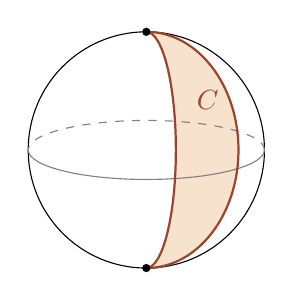
\begin{tikzpicture}[scale=1.5]
  \fill[sand] (0,1) arc[start angle=90, end angle=-90, x radius=0.78, y radius=1]
     arc[start angle=-90, end angle=90, x radius=0.25, y radius=1];
  \draw (0,0) circle (1);
  \draw[gray] (-1,0) arc[start angle=180, end angle=360, x radius=1, y radius=0.25];
  \draw[gray,dashed] (1,0) arc[start angle=0, end angle=180, x radius=1, y radius=0.25];
  \draw[rust,thick] (0,1) arc[start angle=90, end angle=-90, x radius=0.78, y radius=1];
  \draw[rust,thick] (0,1) arc[start angle=90, end angle=-90, x radius=0.25, y radius=1];
  \fill (0,1) circle (1pt); \fill (0,-1) circle (1pt);
  \node[rust] at (0.52,0.42) {$C$};
\end{tikzpicture}
\caption{The event ``$PQ$ misses $I$'' is the lune of longitudes $L>\pi-C$, of angle $C$, which
covers the fraction $\frac{C}{2\pi}$ of the sphere.}
\label{fig:lune}
\end{figure}

On the sphere the miss events become lunes. The side $PQ$ misses $I$ when $z>\rho$, that is when
$s>\frac A2+\frac B2$, or $L>\pi-C$: the lune between the meridians at $\pi-C$ and $\pi$, of angle $C$
(Figure~\ref{fig:lune}). Its area is $\frac{C}{2\pi}$ of the sphere. The three sides give lunes of
angles $A$, $B$, $C$, one on each of three spheres, and as the angles of a triangle they add up to a
hemisphere's worth.

\section{What remains}

The theorem is proved for all radii, but the question as asked is still open: a proof that shows
the $\frac12$ without integrating. Theorem~\ref{thm:sphere} narrows the target. It would be enough to
see, without computation, why the eight-sheeted map $S$ preserves area; or why, in the remark of
Section~4, a side misses as often as the opposite vertex falls inside the incircle.

\paragraph{Verification.} The algebra and calculus of Sections~2 to~5 are formally verified in Lean~4
with Mathlib~\cite{mathlib}: the chord identities, the integral of~\eqref{eq:u} over its whole range
(equal to $\pi$), the density~\eqref{eq:density} and its distribution function, the half-angle
identity behind $A+B+C=\pi$, the final sum, and the folding step of Theorem~\ref{thm:sphere}. The
change of variables~\eqref{eq:jacobian} as a statement about measures, and the plane geometry of
Lemmas~\ref{lem:sectors} and~\ref{lem:miss}, are checked by hand and by simulation: an independent
program confirms Theorem~\ref{thm:main} for four radius triples, the per-side probabilities, the
uniform angle, and the joint law of $(s,v)$. Code and proofs are at
\url{https://github.com/jvvk/mathematics/tree/main/tangent-circles-incentre}.

\paragraph{Acknowledgements.} Dan posed the problem and the two-circle statement, and user170231,
Jack D'Aurizio, dnqxt and Blue contributed to the discussion on Mathematics Stack Exchange.
Anthropic's Claude (Opus~5.5) was used to find the proofs, write the Lean formalisation and the
checking programs, and draft this text. The author checked the proofs and takes responsibility for
the content.

\begin{thebibliography}{9}
\bibitem{DanEqual}
Dan, Random triangle on a ring of three tangent circles (one vertex per circle): what is the
probability that the triangle contains the centre of the ring?, Mathematics Stack Exchange,
question 5084455, 21 July 2025, with the author's answer 5084456,
\url{https://math.stackexchange.com/q/5084455} (accessed 9 October 2026).

\bibitem{user170231}
user170231, answer 5084571 to~\cite{DanEqual}, Mathematics Stack Exchange, 21 July 2025,
\url{https://math.stackexchange.com/a/5084571} (accessed 9 October 2026).

\bibitem{DanAny}
Dan, Random triangle on three mutually tangent circles with centres $A,B,C$: probability that the
triangle contains incentre of $\triangle ABC$ is $1/2$?, Mathematics Stack Exchange, question
5086572, 30 July 2025, \url{https://math.stackexchange.com/q/5086572} (accessed 9 October 2026).

\bibitem{DanLemma}
Dan, The probability that a line segment, whose endpoints are random points on two tangent
circles, crosses a line segment tangent to the circles, Mathematics Stack Exchange, question
5087823, 4 August 2025, \url{https://math.stackexchange.com/q/5087823} (accessed 9 October 2026).

\bibitem{DanMO}
Dan, Random triangle on a ring of three tangent circles: show that the probability that the
triangle contains the centre is 1/2, MathOverflow, question 498968, 9 August 2025,
\url{https://mathoverflow.net/q/498968} (accessed 9 October 2026).

\bibitem{Santalo}
L. A. Santal\'o, \emph{Integral geometry and geometric probability}, Addison-Wesley, Reading, MA
(1976).

\bibitem{mathlib}
The mathlib Community, The Lean mathematical library, in \emph{Proceedings of the 9th ACM SIGPLAN
International Conference on Certified Programs and Proofs (CPP 2020)}, ACM, New York (2020)
pp.~367--381.
\end{thebibliography}

\vspace{1em}
\noindent\textsc{Vamshi Jandhyala}\\
London, United Kingdom
\end{document}
